\chapter{Project planning}
\section{Time schedule}
Below is shown the preliminary time schedule of the project. This schedule will change and must be versionized with every change and updated with regards to time on tasks, tasks and details is okay to add and change.\\ 

\begin{table}[H]
\centering
\begin{tabular}{|l |p{4cm} |c |c |c |c |c|}
\hline 
$\#$ & Task Name & Duration(d) & Start & Finish & Predecessor & Resources \\ 
\hline 
1 & System design & 10 days & 03-feb & 14-feb & none & NG \& JK \\ 
\hline
1-1 & Acceptance test & * & * & * & none &  NG \& JK \\ 
\hline
2 & Technology dev and research & 10 days & 17-feb & 28-feb & $\#$1 & NG \& JK \\ 
\hline 
3 & Development phase & 43 days & 03-mar & 30-apr & $\#$2 & NG \& JK \\ 
\hline 
5 & Finalize documentation & 7 days & 01-may & 9-may & $\#$1,2,3,4 & NG \& JK \\ 
\hline 
6 & Report & 20 days & 5-may & 30-jun & $\#$1,2,3,4,(5) & NG \& JK \\ 
\hline \hline
~ & In total & 85 days & 03-feb & 30-may & ~ & ~ \\ 
\hline 
\end{tabular} 
\end{table}

\begin{figure}[H]
\centering
\includegraphics[width=.9\textwidth]{billeder/timeschedule_vector}
\caption{Time schedule}
\end{figure}

\section{Experiments}
\subsection{Determine the optimal placement for sensors}
A possible extension of the project will be to apply the sensors to a foot and check whether the system works as intended. Before we can apply the sensors to a foot we need to find the optimal placement for the sensors. This can be done with an experiment where we look at heat maps of feet. This experiment will performed by someone other than us but we might use this data to extend our project.

\subsection{Field test of sensor unit}
It will be most natural to apply a sensor unit to a foot to determine the temperature of the foot. This way we will be able to determine if the sensor need to be applied directly to the skin or if they work by close proximity. 

\section{Technologies}
We want to implement a data communication line, bus or protocol. The technology will revolve around using as few wires as possible. 

\section{Project organizing}
This section describes organizing, planning and other practical aspects of the project.

\subsection{Project flow}
The project work shall follow an iterative process were each phase will be repeated several times. The amount of work put into each task can vary from time to time and will be decided by the group members each time depending on how much is needed. Below is shown a figure describing the project flow. If the method and work flow doesn't work as intended the procedure can be altered at all times during the project.
\begin{figure}[H]
\centering
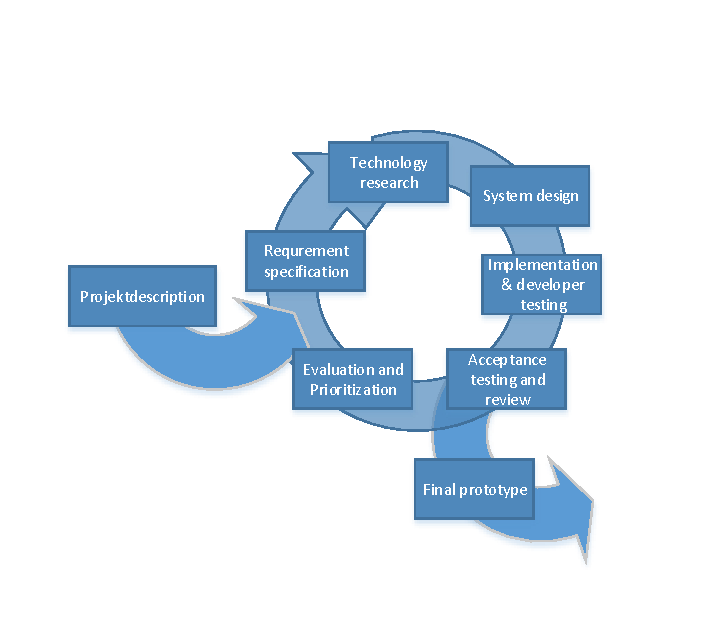
\includegraphics[width=.8\textwidth]{billeder/iteration_vector}
\caption{Figure of the work flow and procedure}
\end{figure}
One iteration will vary in time but must not exceed 3 weeks to ensure the agile development method.\\

\subsection{Meetings}
The project is divided into sprints of 1 week duration. This is to help ensure momentum and agility.\\
Supervisor meetings: A minimum of one per week, preferably the same weekday: suggestion Monday.\\
Daily group meetings: A minimum of 3 per week, preferably more. Suggestion: Tuesday, Wednesday and Friday.

\subsubsection{Weekly supervisor meetings agenda}
\textit{This agenda is a guideline and may vary if the group see fit.}
\begin{itemize}
\item Since last meeting
\item Next weeks goals
\item Workrelated subjects
\item Closing remarks
\end{itemize}

\subsubsection{Daily group meetings agenda}
\textit{This agenda is a guideline and may vary if the group see fit.}
\begin{itemize}
\item What did I accomplish yesterday?
\item What will I do today?
\subitem $\circ$ Todays "Must-Win" battles?
\item What obstacles are impeding my progress?
\end{itemize}

\subsection{Work and task distribution}
All tasks and challenges related to the project must be noted on posted notes and hung on the project planning board. This board must be organized to help give an overview of the projects progress and future task.\\
Task distribution will, whenever possible, be allocated at the daily group meetings. It is at all times possible to add tasks to the board.\\

